\documentclass[14pt]{extbook}
\usepackage{multicol, enumerate, enumitem, hyperref, color, soul, setspace, parskip, fancyhdr} %General Packages
\usepackage{amssymb, amsthm, amsmath, latexsym, units, mathtools} %Math Packages
\everymath{\displaystyle} %All math in Display Style
% Packages with additional options
\usepackage[headsep=0.5cm,headheight=12pt, left=1 in,right= 1 in,top= 1 in,bottom= 1 in]{geometry}
\usepackage[usenames,dvipsnames]{xcolor}
\usepackage{dashrule}  % Package to use the command below to create lines between items
\newcommand{\litem}[1]{\item#1\hspace*{-1cm}\rule{\textwidth}{0.4pt}}
\pagestyle{fancy}
\lhead{Progress Quiz 10}
\chead{}
\rhead{Version A}
\lfoot{5170-5105}
\cfoot{}
\rfoot{Summer C 2021}
\begin{document}

\begin{enumerate}
\litem{
Which of the following equations \textit{could} be of the graph presented below?
\begin{center}
    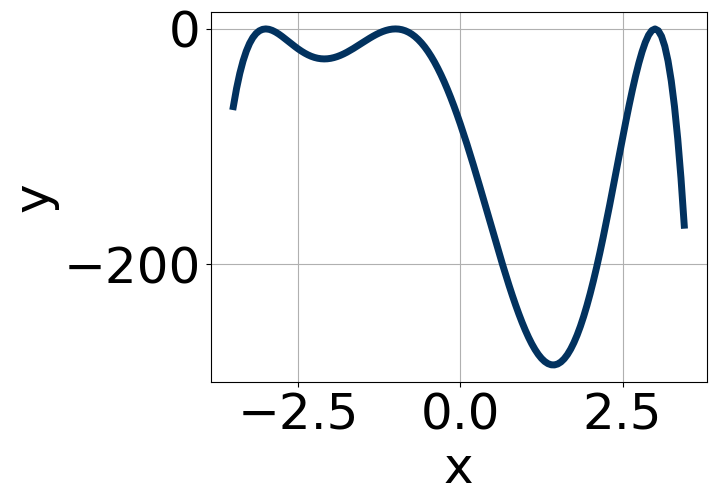
\includegraphics[width=0.5\textwidth]{../Figures/polyGraphToFunctionA.png}
\end{center}
\begin{enumerate}[label=\Alph*.]
\item \( -18(x + 3)^{6} (x + 1)^{4} (x - 3)^{8} \)
\item \( 12(x + 3)^{8} (x + 1)^{4} (x - 3)^{7} \)
\item \( -7(x + 3)^{6} (x + 1)^{10} (x - 3)^{7} \)
\item \( 8(x + 3)^{6} (x + 1)^{6} (x - 3)^{6} \)
\item \( -12(x + 3)^{10} (x + 1)^{11} (x - 3)^{5} \)

\end{enumerate} }
\litem{
Describe the end behavior of the polynomial below.\[ f(x) = -9(x + 8)^{2}(x - 8)^{5}(x - 6)^{2}(x + 6)^{3} \]\begin{enumerate}[label=\Alph*.]
\begin{multicols}{2}\item 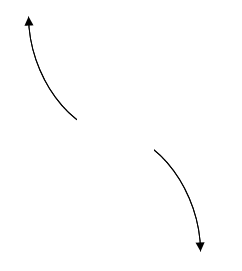
\includegraphics[width = 0.3\textwidth]{../Figures/polyEndBehaviorAA.png}\item 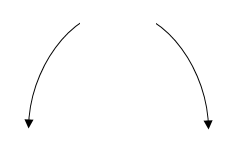
\includegraphics[width = 0.3\textwidth]{../Figures/polyEndBehaviorBA.png}\item 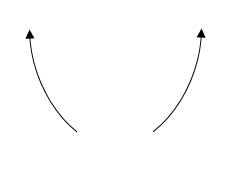
\includegraphics[width = 0.3\textwidth]{../Figures/polyEndBehaviorCA.png}\item 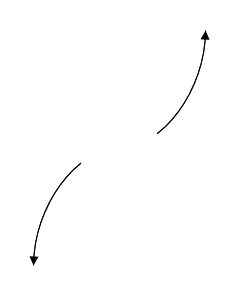
\includegraphics[width = 0.3\textwidth]{../Figures/polyEndBehaviorDA.png}\end{multicols}\item None of the above.
\end{enumerate} }
\litem{
Construct the lowest-degree polynomial given the zeros below. Then, choose the intervals that contain the coefficients of the polynomial in the form $x^3+bx^2+cx+d$.\[ 4 + 3 i \text{ and } 1 \]\begin{enumerate}[label=\Alph*.]
\item \( b \in [1, 2], c \in [-6, -4.35], \text{ and } d \in [3.48, 4.06] \)
\item \( b \in [1, 2], c \in [-4.24, -2.63], \text{ and } d \in [2.96, 3.37] \)
\item \( b \in [-17, -7], c \in [31.51, 33.82], \text{ and } d \in [-25.2, -24.86] \)
\item \( b \in [8, 10], c \in [31.51, 33.82], \text{ and } d \in [24.44, 25.5] \)
\item \( \text{None of the above.} \)

\end{enumerate} }
\litem{
Which of the following equations \textit{could} be of the graph presented below?
\begin{center}
    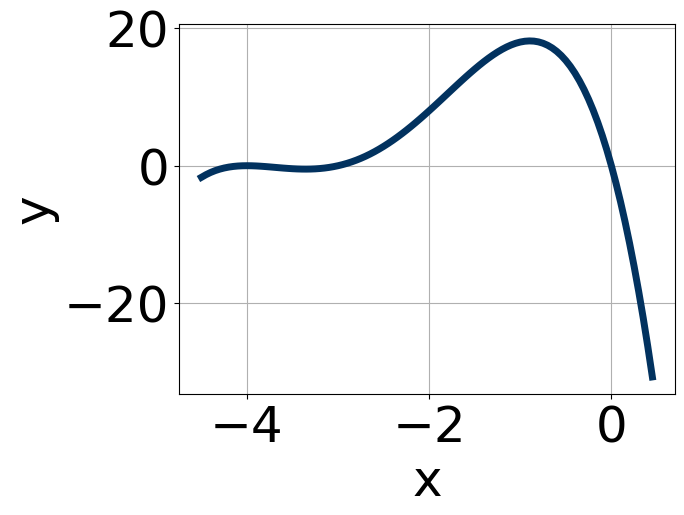
\includegraphics[width=0.5\textwidth]{../Figures/polyGraphToFunctionCopyA.png}
\end{center}
\begin{enumerate}[label=\Alph*.]
\item \( -5x^{5} (x + 4)^{8} (x + 3)^{7} \)
\item \( -19x^{6} (x + 4)^{6} (x + 3)^{7} \)
\item \( -14x^{10} (x + 4)^{9} (x + 3)^{5} \)
\item \( 10x^{11} (x + 4)^{8} (x + 3)^{10} \)
\item \( 19x^{11} (x + 4)^{4} (x + 3)^{7} \)

\end{enumerate} }
\litem{
Describe the zero behavior of the zero $x = 8$ of the polynomial below.\[ f(x) = -9(x - 6)^{9}(x + 6)^{6}(x - 8)^{12}(x + 8)^{9} \]\begin{enumerate}[label=\Alph*.]
\begin{multicols}{2}\item 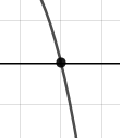
\includegraphics[width = 0.3\textwidth]{../Figures/polyZeroBehaviorCopyAA.png}\item 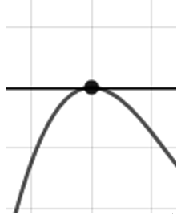
\includegraphics[width = 0.3\textwidth]{../Figures/polyZeroBehaviorCopyBA.png}\item 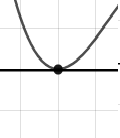
\includegraphics[width = 0.3\textwidth]{../Figures/polyZeroBehaviorCopyCA.png}\item 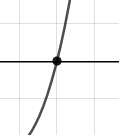
\includegraphics[width = 0.3\textwidth]{../Figures/polyZeroBehaviorCopyDA.png}\end{multicols}\item None of the above.
\end{enumerate} }
\litem{
Construct the lowest-degree polynomial given the zeros below. Then, choose the intervals that contain the coefficients of the polynomial in the form $ax^3+bx^2+cx+d$.\[ \frac{3}{2}, 5, \text{ and } \frac{-4}{3} \]\begin{enumerate}[label=\Alph*.]
\item \( a \in [0, 10], b \in [45, 52], c \in [97, 103], \text{ and } d \in [55, 64] \)
\item \( a \in [0, 10], b \in [-34, -27], c \in [-9, -4], \text{ and } d \in [55, 64] \)
\item \( a \in [0, 10], b \in [-34, -27], c \in [-9, -4], \text{ and } d \in [-66, -56] \)
\item \( a \in [0, 10], b \in [26, 37], c \in [-9, -4], \text{ and } d \in [-66, -56] \)
\item \( a \in [0, 10], b \in [-13, -7], c \in [-76, -68], \text{ and } d \in [-66, -56] \)

\end{enumerate} }
\litem{
Construct the lowest-degree polynomial given the zeros below. Then, choose the intervals that contain the coefficients of the polynomial in the form $x^3+bx^2+cx+d$.\[ -3 + 2 i \text{ and } 2 \]\begin{enumerate}[label=\Alph*.]
\item \( b \in [-5.5, -1.2], c \in [-3, 3], \text{ and } d \in [24, 27] \)
\item \( b \in [0.7, 1.5], c \in [-6, -3], \text{ and } d \in [0, 9] \)
\item \( b \in [3.8, 5.3], c \in [-3, 3], \text{ and } d \in [-32, -24] \)
\item \( b \in [0.7, 1.5], c \in [-3, 3], \text{ and } d \in [-10, -3] \)
\item \( \text{None of the above.} \)

\end{enumerate} }
\litem{
Construct the lowest-degree polynomial given the zeros below. Then, choose the intervals that contain the coefficients of the polynomial in the form $ax^3+bx^2+cx+d$.\[ \frac{-3}{5}, \frac{-7}{2}, \text{ and } \frac{-3}{2} \]\begin{enumerate}[label=\Alph*.]
\item \( a \in [15, 23], b \in [110, 119], c \in [165, 169], \text{ and } d \in [-64, -58] \)
\item \( a \in [15, 23], b \in [-117, -109], c \in [165, 169], \text{ and } d \in [-64, -58] \)
\item \( a \in [15, 23], b \in [110, 119], c \in [165, 169], \text{ and } d \in [54, 68] \)
\item \( a \in [15, 23], b \in [-53, -49], c \in [-85, -80], \text{ and } d \in [54, 68] \)
\item \( a \in [15, 23], b \in [88, 93], c \in [36, 51], \text{ and } d \in [-64, -58] \)

\end{enumerate} }
\litem{
Describe the zero behavior of the zero $x = 7$ of the polynomial below.\[ f(x) = 2(x + 7)^{7}(x - 7)^{10}(x - 3)^{4}(x + 3)^{8} \]\begin{enumerate}[label=\Alph*.]
\begin{multicols}{2}\item 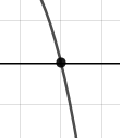
\includegraphics[width = 0.3\textwidth]{../Figures/polyZeroBehaviorAA.png}\item 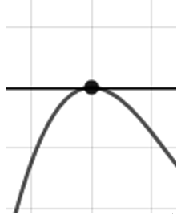
\includegraphics[width = 0.3\textwidth]{../Figures/polyZeroBehaviorBA.png}\item 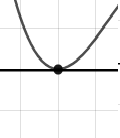
\includegraphics[width = 0.3\textwidth]{../Figures/polyZeroBehaviorCA.png}\item 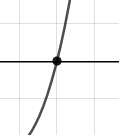
\includegraphics[width = 0.3\textwidth]{../Figures/polyZeroBehaviorDA.png}\end{multicols}\item None of the above.
\end{enumerate} }
\litem{
Describe the end behavior of the polynomial below.\[ f(x) = -3(x + 4)^{3}(x - 4)^{6}(x - 5)^{5}(x + 5)^{7} \]\begin{enumerate}[label=\Alph*.]
\begin{multicols}{2}\item 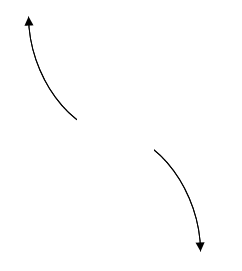
\includegraphics[width = 0.3\textwidth]{../Figures/polyEndBehaviorCopyAA.png}\item 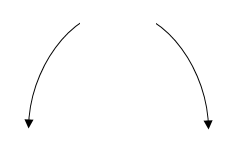
\includegraphics[width = 0.3\textwidth]{../Figures/polyEndBehaviorCopyBA.png}\item 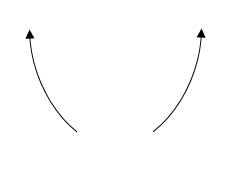
\includegraphics[width = 0.3\textwidth]{../Figures/polyEndBehaviorCopyCA.png}\item 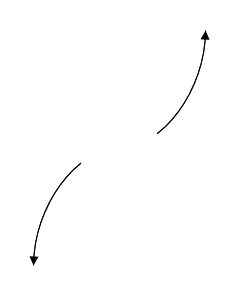
\includegraphics[width = 0.3\textwidth]{../Figures/polyEndBehaviorCopyDA.png}\end{multicols}\item None of the above.
\end{enumerate} }
\end{enumerate}

\end{document}